%\documentclass[12pt, openright,oneside, a4paper, english, brazil]{abntex2}
\documentclass[12pt,
               openright,
               oneside,
               a4paper,
							 section=TITLE,     % COMO SÃO AS LETRAS MAIÚSCULAS EM SEÇÃO
               subsection=Title,  % EM DIANTE ESCRITO NORMALMENTE
               english,brazil]{article}

% ----------------------------
% Pacotes básicos 
% ----------------------------
% Referências
\usepackage[brazilian,hyperpageref]{}	
\usepackage{hyperref}
\usepackage[alf]{abntex2cite}			

% Fonte e codificação (acentuação)
\usepackage{lmodern}       
\renewcommand{\sfdefault}{ppl}
\usepackage[T1]{fontenc}	
\usepackage[utf8]{inputenc}	
% Tabelas e Figuras
\usepackage{ctable}             
\usepackage{multirow}
\usepackage{array}
\usepackage{float}              
\usepackage{longtable}          
\usepackage{xcolor,colortbl}    
\usepackage{booktabs}           
\usepackage{graphicx}			
\usepackage{subfig}             
\usepackage{caption}            
\usepackage{epstopdf}           

% Equações e símbolos
\usepackage{amsmath}            
\usepackage{nomencl} 
\usepackage{cleveref} 
\usepackage{calrsfs}
\usepackage{amssymb}
\usepackage{psfrag}
\usepackage[brazil]{babel}
% Texto
%\usepackage[showframe,heightrounded]{geometry}
\usepackage{geometry}
\usepackage{indentfirst}		
\usepackage{color}				
\usepackage{microtype} 			
\usepackage{lastpage}			
\usepackage{enumitem}                % Para os itens em letras
\usepackage{lipsum}
\usepackage{lastpage}
\usepackage{tablefootnote}
\usepackage{pdflscape}
\usepackage{scalefnt}
\usepackage[stable]{footmisc}
% ----------------------------------------------------------
% Configurações do texto
% ----------------------------------------------------------

% Recuo do parágrafo :
\setlength{\parindent}{1.5cm}
\setlength{\parskip}{0cm} 
\geometry{a4paper}%,left=3cm,right=2cm,top=3cm,bottom=2cm} % SEMPRE BOM VER A DOCUMENTAÇÃO
\hoffset = -1in
\voffset = -1in
\oddsidemargin = 1.5cm
\topmargin = 2cm
\headheight = 0pt
\headsep = 6pt % multiplicar por 0.03515 para obter cm
\textheight = 249mm
\textwidth = 18cm
\marginparsep = 0pt
\marginparwidth = 0pt
\footskip = 6mm
%
%
%
\usepackage{array}
\newcolumntype{L}[1]{>{\raggedright\let\newline\\\arraybackslash\hspace{0pt}}m{#1}}
\newcolumntype{C}[1]{>{\centering\let\newline\\\arraybackslash\hspace{0pt}}m{#1}}
\newcolumntype{R}[1]{>{\raggedleft\let\newline\\\arraybackslash\hspace{0pt}}m{#1}}
%
%
%
\newtheorem{teorema}{Teorema}[section]
\newtheorem{propriedade}[teorema]{Condição}
\newtheorem{lema}[teorema]{Lema}
\newtheorem{corolario}[teorema]{Corolário}
\newtheorem{proposicao}[teorema]{Proposição}
\newtheorem{definicao}[teorema]{Definição}
\newtheorem{exemplo}[teorema]{Exemplo}
\newtheorem{af}[teorema]{AF}
\newtheorem{exercicio}[teorema]{Exercício}
\newtheorem{algoritmo}{Algoritmo}[section]
\newtheorem{exc}{}[section]
\newtheorem{impl}{}[section]
\newtheorem{hip}{H\hspace{-.12cm}}
\newtheorem{res}{R\hspace{-.12cm}}
%
%
%
\newcommand{\rel}{\Bbb R^{\ell}}
\newcommand{\rell}{\mathbb R^{\ell}_{+}}
\newcommand{\rr}{\mathbb R}
\newcommand{\bb}[1]{\boldsymbol{#1}}
\newcommand{\ol}[1]{\overline{#1}}
\newcommand{\hess}{\nabla^2(f(\bb{x}))}

\newcommand{\kktmax}[3]{
\begin{aligned}
& \underset{#1}{\text{maximizar}}
& & {#2} \\
& \text{sujeito a} 
& & {#3} \\
\end{aligned}}

\newcommand{\kktmin}[3]{
\begin{aligned}
& \underset{#1}{\text{minimizar}}
& & {#2} \\
& \text{sujeito a} 
& & {#3} \\
\end{aligned}}

%  Novos macros
\newcommand{\R}{\mathbb{R}}
\newcommand{\N}{\mathbb{N}}
\newcommand{\U}{\mathcal{U}}
\newcommand{\Rn}{{\R}^n}
\newcommand{\sumin}{\sum_{i=1}^n}
\newcommand{\Rl}{{\R}^\ell}
\newcommand{\Rm}{{\R}^m}
\newcommand{\ind}{1,\ldots,n}
%
%
%
%
%

\title{Análise dos determinantes da probabilidade de um jornalista ter sido assassinado em serviço}
\author{Pedro Milreu Cunha \thanks{Mestrando/Doutorando PPGE/UFPB}}

\date{}
%
%
%
%
%
%
%
%
%
\begin{document}
\topmargin = 0.2cm
\maketitle

\setlength{\parindent}{0cm}



\textbf{RESUMO:} O presente trabalho teve o intuito de analisar a importância de um conjunto de variáveis que capturam características pessoais e profissionais de uma amostra de jornalistas no que tange à probabilidade de um jornalista ser assassinado em razão de seu trabalho. Para tanto, foram utilizados o modelo Probit homocedástico tradicional e também um modelo heterocedástico. Os resultados obtidos foram bastante significativos, com o local de atuação sendo o Brasil e a condição de ser não-estrangeiro aumentando a probabilidade da morte de um jornalista ter sido um assassinato, enquanto trabalhar como \textit{freelancer}, ser homem e cobrir tópicos envolvendo política ou guerra diminuem essa probabilidade. Por fim, quando as suspeitas sobre a morte recaem sobre oficiais militares, há uma redução bastante significativa da probabilidade de ter sido um assassinato.

\textbf{Palavras-chave}: Jornalistas. Assassinatos. Probit.

\textbf{JEL:} C25. J28.

\vspace{0.6cm}

\textbf{ABSTRACT:} The aim of this paper was to analyze the importance of a set of variables that capture personal and profissional characteristics of a sample of journalists with respect to the probability of a journalist being murdered due to his work. For this, both the traditional homocedastic Probit model and the heterocedastic model were used. The results obtained were quite significant, with the country of work being Brazil and the condition of being a non-foreigner increasing the probability of the death of a journalist having been a murder, while acting as \textit {freelancer}, being a man and covering topics involving politics or war lessens that likelihood. Finally, when suspicions about the death fall on military officers, there is a very significant reduction in the likelihood that it was a murder.

\textbf{Keywords}: Journalists. Murders. Probit.

\textbf{JEL:} C25. J28.

\newpage
\topmargin = 2cm
\setlength{\parindent}{1.5cm}

\section{Introdução}

De acordo com dados do \textit{Committee to Protect Journalists} (CPJ), organização não governamental estadunidense independente e sem fins lucrativos que visa promover a liberdade de imprensa e defender os direitos dos jornalistas, 1397 profissionais foram mortos entre 1992 e 2020 em decorrência de seu trabalho, conforme pode ser visto na figura \ref{fig:serie_historica}.

\begin{figure}[H]
	\centering
	\caption{Série histórica - mortes confirmadas$^*$ de jornalistas }
	\label{fig:serie_historica}
	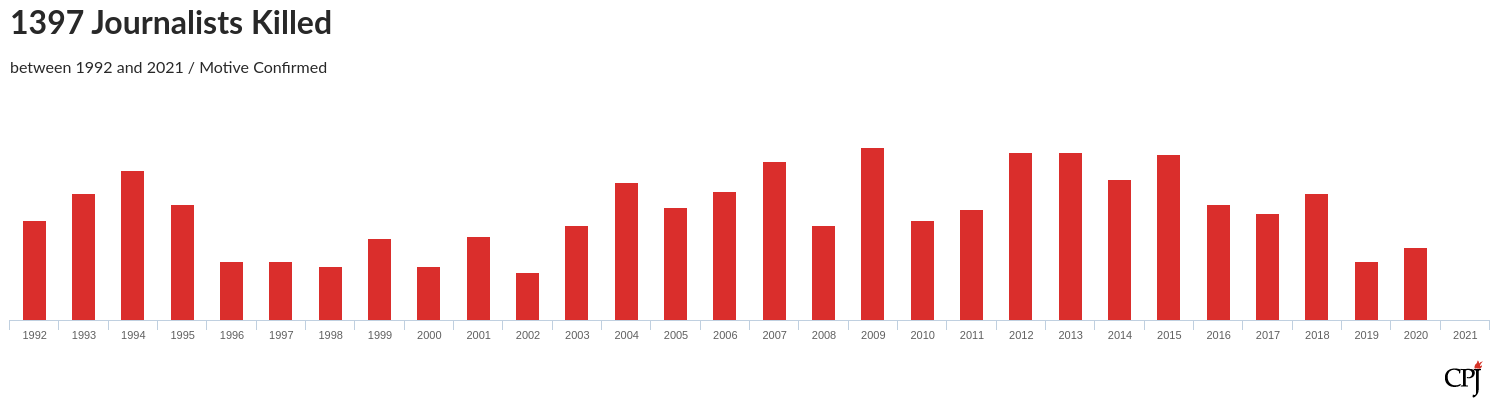
\includegraphics[width=\linewidth]{"Figuras/serie_mortes.png"} \\
\caption*{Fonte: \cite{CPJ2020}.}
\end{figure}

A organização separa as mortes em três categorias:
\begin{enumerate}
    \item Mortes em represália direta ao trabalho do(a) jornalista;
    
    \item Mortes em decorrência de fogo cruzado/combate;
    
    \item Mortes em decorrência de atribuições/missões perigosas.
\end{enumerate}

Para o presente trabalho, o foco recai sobre a primeira categoria, buscando analisar quais fatores afetam a probabilidade de um jornalista morrer diretamente devido à repercussão de seu trabalho e não por acidente ou "azar" (fogo cruzado).

A importância de se estudar esse tópico dá-se pelo grande papel influenciador que a mídia tem na sociedade, de modo que não apenas a questão individual das mortes é problemática, mas também o contexto maior, isto é, a repressão sistemática da imprensa livre e a violência contra os profissionais desse setor. Conforme apontam os autores em \citeonline{Coyne2004}, o sucesso do desenvolvimento econômico  é caracterizado por coordenação generalizada. Nesse sentido, a mídia tem papel pivotal nas mudanças de jogos de conflito da economia para jogos de cooperação.

Para além disso, a mídia também tem um papel indireto, ao afetar a percepção dos indivíduos acerca de diversos acontecimentos que os rodeiam, como por exemplo ataques terroristas. \citeonline{Keinan2003} realizaram um estudo em Israel, após uma série de graves atentados terroristas. Os autores apontam que os efeitos da cobertura jornalista detalhada dos eventos causou efeitos semelhantes aos sentidos por pessoas com Estresse Pós-Traumático, condição associada com perda de produtividade e custos econômicos (\cite{Ferry2015}, \cite{Olesen2011}).

Contextualizada a importância da mídia e dos jornalistas, o presente artigo busca entender quais fatores afetam a probabilidade de um jornalista ser assassinado em direta represália ao seu trabalho, considerando apenas a amostra de jornalistas que foram mortos entre 1992 e 2020, disponibilizada pelo \cite{CPJ2020}.

Considerando o local de atuação do profissional, os resultados obtidos apontam que atuar no Brasil aumenta significativamente a probabilidade de um jornalista ser assassinado em represália direta ao seu trabalho. Além disso, não ser estrangeiro onde atua também aumenta essa chance. Por outro lado, trabalhar como \textit{freelancer}, ser homem e cobrir temas que envolvem política ou guerra reduzem a probabilidade da morte do profissional ter sido um assassinato. Finalmente, quando a suspeita da morte se dá nos oficiais do governo ou militares, a chance de ter sido um assassinato também cai.

O restante do artigo está dividido em três seções: i) Metodologia, onde são apresentados a fonte de dados e as estatísticas descritivas, os dois modelos Probit e os modelos empíricos estimados; ii) Resultados, seção na qual são discutidos os resultados obtidos no trabalhos e iii) Considerações finais, onde são consolidados os principais resultados do artigo e apontadas as possíveis melhoras e caminhos futuros.

\section{Metodologia}

\subsection{Fonte de dados e estatísticas descritivas}

Todos as variáveis utilizadas foram criadas à partir dos dados obtidos em \cite{CPJ2020}. A tabela seguir apresenta o nome e a descrição de cada variável utilizada:

\begin{table}[H]
\centering
\scalefont{0.75}
\caption{Descrição das  variáveis}
\label{tab:dados}
\begin{tabularx}{\textwidth}{lc} \\
Variável &  Descrição \\ \midrule
Assassinato  & Variável binária que assume valor $1$ caso o jornalista tenha sido assassinado \\ 
Brasil & Variável binária que assume valor $1$ caso o jornalista atuasse no Brasil \\  
\textit{Freelancer} & Variável binária que assume valor $1$ caso o jornalista atuasse como \textit{freelancer}\\ Governo & Variável binária que assume valor $1$ caso o suspeito de assassinato seja relacionado ao governo \\ Guerra & Variável binária que assume valor $1$ caso guerra fosse um dos tópicos de cobertura do jornalista \\ Homem & Variável binária que assume valor $1$ caso o jornalista fosse homem \\ Militares & Variável binária que assume valor $1$ caso o suspeito de assassinato seja relacionado aos militares \\ Não-estrangeiro & Variável binária que assume valor $1$ caso o jornalista não fosse estrangeiro no país onde atuava \\ Política & Variável binária que assume valor $1$ caso política fosse um dos tópicos de cobertura do jornalista  \\ \bottomrule 
\end{tabularx}
\caption*{Fonte: Elaboração própria à partir dos dados disponíveis em \cite{CPJ2020}.}
\end{table}

Em seguida, na tabela $\ref{tab:descritivas}$, são apresentadas as estatísticas descritivas das variáveis utilizadas na estimação:

\begin{table}[H] \centering 
  \caption{Estatísticas descritivas} 
  \label{tab:descritivas} 
\begin{tabular}{lccccccc} 
Estatística & \multicolumn{1}{c}{N} & \multicolumn{1}{c}{Média} & \multicolumn{1}{c}{Desv.pad.} & \multicolumn{1}{c}{Mín} & \multicolumn{1}{c}{$\mathcal{P}_{25}$} & \multicolumn{1}{c}{$\mathcal{P}_{75}$} & \multicolumn{1}{c}{Máx} \\ 
\midrule
Assassinato & 1160 & 0,612 & 0,487 & 0 & 0 & 1 & 1 \\ 
Brasil & 1160 & 0,034 & 0,180 & 0 & 0 & 0 & 1 \\ 
Governo & 1160 & 0,189 & 0,392 & 0 & 0 & 0 & 1 \\ 
Militares & 1160 & 0,231 & 0,422 & 0 & 0 & 0 & 1 \\ 
Política & 1160 & 0,388 & 0,487 & 0 & 0 & 1 & 1 \\ 
Homem & 1160 & 0,930 & 0,255 & 0 & 1 & 1 & 1 \\ 
Não-estrangeiro & 1160 & 0,879 & 0,326 & 0 & 1 & 1 & 1 \\ 
\textit{Freelancer} & 1160 & 0,197 & 0,398 & 0 & 0 & 0 & 1 \\ 
Guerra & 1160 & 0,433 & 0,496 & 0 & 0 & 0 & 1 \\ 
\bottomrule \\ 
\end{tabular} 
\caption*{Fonte: Elaboração própria.}
\end{table} 

Como se pode observar, considerando as 1160 mortes confirmadas de jornalistas\footnote[1]{O \textit{Committee to Protect Journalists} (CPJ) considera um caso  "confirmado" como relacionado ao trabalho apenas quando razoávelmente certo de que o jornalista foi assassinado em represália direta ao seu trabalho; em combate ou fogo cruzado; ou enquanto realizando tarefa perigosa \cite{CPJ2020}.}, tem-se que $61,2\%$ delas são consideradas assassinatos. Além disso, $3,4\%$ dos profissionais atuavam no Brasil, $93\%$ eram homens, $87,9\%$ não eram estrangeiros e $19,7\%$ atuavam como \textit{freelancers}.

Considerando os tópicos de cobertura, $22,6\%$ atuavam cobrindo exclusivamente guerra e $37,3$ apenas política. Por fim, no que tange à suspeita de cometer o crime, em $16,7\%$ dos casos ela recai sobre o governo e em $21,6\%$ sobre os militares.

\subsection{Modelo \textit{Probit}\footnote[2]{Essa seção baseia-se largamente em \cite{Greene2018}.}}

Utilizou-se o modelo probit para analisar quais variáveis impactam significativamente na probabilidade de um jornalista ser assassinado enquanto trabalha. Considere uma variável aleatória latente
$$
Y^* = X^{T} \cdot \beta + \epsilon
$$
, na qual $\beta$ é um vetor de parâmetros. Essa variável não é observável; tudo que pode ser visto é a ocorrência ou não de um evento, sendo isso representado pela variável binária $Y$, que assume valor $1$ no caso de ocorrência e $0$ caso contrário.  Dessa forma, o que de fato é observado é que:
$$
\begin{cases}
Y = 1, \text{ se } Y^* = X^T \cdot \beta + \epsilon > 0 \\
Y = 0, \text{ caso contrário}
\end{cases}
$$

Portanto,
$$
P(Y = 1 | X) = P(Y^* > 0 | X) = P(\epsilon > -X^T \cdot \beta | X)
$$

Para o caso do modelo probit, é feita a suposição de que $\epsilon \sim \mathcal{N}(0, 1)$, ou seja, assume-se como hipótese simplificadora que o termo erro segue uma distribuição normal padrão com média $0$ e variância unitária\footnote[3]{Esse é um ponto importante e é o que distingue o modelo Probit tradicional do modelo Probit heterocedástico, abordado na proxima subseção.}. 

Uma vez que a distribuição normal é simétrica, a expressão acima pode ser reescrita como
\begin{equation}
P(Y = 1 | X) = P(\epsilon < X^T \cdot \beta) = \Phi(X^T \cdot \beta)    
\end{equation}

Tecnicamente, a expressão correta é
$$
P(Y = 1 | X) = \Phi \left( \frac{X^T \cdot \beta}{\sigma} \right)
$$
onde $\sigma$ é o desvio-padrão do termo de erro. Fazendo uso da suposição simplificadora $\sigma = 1$, chega-se na equação $(1)$.

A equação $(1)$ é usualmente estimada pelo método da Máxima Verossimilhança\footnote[4]{O método de estimação por Máxima Verossimilhança consiste em maximizar uma função de verossimilhança, de forma que, considerando o modelo estatístico utilizado, os dados observados sejam os mais prováveis. Embora em alguns casos uma solução analítica seja possível (por exemplo nos Mínimos Quadrados Ordinários (MQO)), geralmente será necessária uma solução numérica. }. Supondo que cada observação $Y_1, Y_2, \dots Y_n \in Y$ seja tratada como um sorteio único de uma distribuição de Bernoulli, o modelo com probabilidade de sucesso $\mathcal{F}(X^T \cdot \beta)$ e distribuição independentes, terá uma função de probabilidade conjunta ou de verossimilhança dada por
\begin{equation}
    P(Y_1 = y_1, Y_2 = y_2, \dots Y_n = y_n | X) = \prod_{y_i=0}[1-\mathcal{F}(X^T \cdot \beta)] \prod_{y_i=1}\mathcal{F}(X^T \cdot \beta)
\end{equation}

Considerando a amostra com $n$ elementos, pode-se simplificar a equação acima para
\begin{equation}
\mathcal{L}(\beta | \text{dados}) = \prod_{i=1}^n [\mathcal{F}(X^T \cdot \beta)]^{y_i} \cdot [1- \mathcal{F}(X^T \cdot \beta)]^{1-y_i}
\end{equation}

Aplicando o logaritmo natural, obtém-se a $\log$ verossimilhança:
\begin{equation}
\ln \mathcal{L} = \sum_{i=1}^n \{ y_i \cdot \ln \mathcal{F}(X^T \cdot \beta) + (1-y_i) \cdot \ln [1 - \mathcal{F}(X^T \cdot \beta)\}
\end{equation}
que é utilizada por facilitar as operações matemáticas necessárias para maximização da verossimilhança.

Para realizar a maximização, deriva-se $(4)$ em relação ao vetor de parâmetros $\beta$ e iguala-se o resultado a zero:
\begin{equation}
\frac{\partial \ln \mathcal{L}}{\partial \beta} = \sum_{i=1}^n \left[ y_i \cdot \frac{\mathcal{G}_i}{\mathcal{F}_i} + (1-y_i) \cdot \frac{(-\mathcal{G}_i)}{(1-\mathcal{F}_i)} \right] \cdot X = 0
\end{equation}
onde $\mathcal{G}(\dot) = \frac{\operatorname{d} \mathcal{G}(\cdot)}{\operatorname{d} X^T \cdot \beta}$.

Naturalmente, para o caso do modelo Probit, $\mathcal{F}(\cdot)$ é a F.D.A. de uma normal padrão com média $0$ e variância $1$, $\Phi(\cdot)$, sendo, portanto, $\mathcal{G}(\cdot) = \phi(\cdot)$, ou seja, a função de densidade normal.

À partir da equação $(1)$, nota-se outra peculiaridade do modelo em questão. Como a relação entre os preditores e a variável de interesse não é linear, ou seja, como o efeito marginal das variáveis independentes muda de acordo com seus respectivos níveis,  a interpretação dos coeficientes deixa de ser direta. Matematicamente, a relação entre $Y$ e os regressores $X$ agora é mediada pela função intermediária $\Phi(\cdot)$.

Deste modo, para calcular-se o efeito esperado de uma mudança em algum regressor binário (variável \textit{dummy}) na probabilidade de ocorrência do evento, procede-se da seguinte maneira:

\begin{itemize} \item Calcula-se o valor previsto da probabilidade de que $Y=1$ para o conjunto original de valores $X$; 

\item Calcula-se o valor prevista do probabilidade de que $Y=1$ para o conjunto novo de valores $X + \Delta X$; \item Calcula-se a diferença entre as duas probabilidades. 
\end{itemize}

Suponha, por exemplo, que $X_k$ seja uma variável categórica que assume valor $1$ quando o indivíduo pertence a um grupo e $0$ caso contrário. Para verificar o impacto do pertencimento a esse grupo na probabilidade de $Y=1$, realiza-se o seguinte processo: 
\begin{itemize} \item Calcula-se o valor previsto para a probabilidade de que $Y=1$ considerando $X_k=1$ e as demais variáveis do vetor $X$ assumindo um valor desejado qualquer $X^*$; 

\item Calcula-se o valor previsto para a probabilidade de que $Y=1$ considerando $X_k=0$ com as demais variáveis do vetor $X=X^*$ inalteradas; 

\item Calcula-se a diferença entre as duas probabilidades. \end{itemize}

Para variáveis contínuas, considerando variações infinitesimais, tem-se que o efeito marginal de um regressor é dado por 
$$ \frac{\partial P(Y=1) }{\partial X_i} = \Phi'(X^T \cdot \beta) \cdot \beta_i = \phi(X^T \cdot \beta) \cdot \beta_i $$. 

Como o efeito varia de acordo com o indivíduo, usualmente estima-se o mesmo considerando um indivíduo médio ou considerando a média de todos os efeitos marginais individuais (sendo essa a opção adotada no presente trabalho).

Em seguida, apresenta-se uma extensão ao modelo Probit tradicional, ao permitir que a variância do termo de erro deixe de ser constante.

\subsection{Modelo \textit{Probit} heterocedástico}

Suponha que em vez de considerar que o termo de erro, $\epsilon$, segue uma distribuição normal padrão com média $0$ e variância $1$, como é feito no modelo Probit tradicional, assuma-se agora que seu desvio-padrão seja da seguinte forma
\begin{equation}
\sigma = \exp(Z^T \cdot \gamma)
\end{equation}
, onde $Z$ é um vetor de variáveis potencialmente diferente de $X$, não contendo ao menos o termo constante e $\gamma$ é um vetor de parâmetros. Essa abordagem é discutida em \citeonline{Freeman2015} e é baseada em \cite{Harvey1976}.

Desse modo, de forma semelhante a equação $(1)$, tem-se que para o modelo heterocedástico,
\begin{equation}
P(Y=1|X) = \Phi \left( \frac{X^T \cdot \beta}{\exp(Z^T \cdot \gamma)}\right)
\end{equation}

Assumindo que as condições de identificabilidade e estimação sejam satisfeitas\footnote[5]{O leitor interessado pode consultar as fontes citadas}, procede-se à estimação utilizando novamente o método da máxima verossimilhança, à partir da equação a seguir:
\begin{equation}
\ln \mathcal{L}(\beta, \gamma) = \sum_{i=1}^n \left\{y_i \cdot \ln \Phi \left( \frac{X^T \cdot \beta}{\exp(Z^T \cdot \gamma)} \right) + (1-y_i) \cdot \ln \Phi \left( 1 - \frac{X^T \cdot \beta}{\exp(Z^T \cdot \gamma)} \right) \right\}
\end{equation}

Entretanto, é preciso cautela pois a presença de heterocedasticidade também afeta a estimação dos efeitos marginais das variáveis explicativas. Notadamente, conforme aponta \citeonline{Greene2018}, para uma variável $w_k$ que pode estar tanto em $X$ quanto em $Z$, é verdade que
\begin{equation}
\frac{\partial P(Y=1 |X,Z)}{\partial w_k} = \left\{ \phi \left[ \frac{X^T \cdot \beta}{\exp(Z^T \cdot \gamma)}\right] \cdot \frac{1}{\exp(Z^T \cdot \gamma)} \right\} \cdot [\beta_k - (X^T \cdot \beta)\gamma_k]   
\end{equation}
onde apenas o primeiro termo (segundo) se aplica se $w_k$ aparecer somente em $X$ ($Z$).

Por fim, considerando que $\gamma = 0$ indica homocedasticidade, pode-se testar para a presença de heterocedasticidade utilizando um teste de razão de verossimilhança (LR), comparando os modelos homo e heterocedásticos\footnote[6]{Outras opções são o teste do Multiplicador de Lagrange (LM) e o teste de Wald. Todos apresentam os mesmo resultados assintóticamente.}. Além disso, pode-se utilizar também o \textit{Akaike Information Criteria} (AIC) e o \textit{Bayesian Information Criteria} (BIC) como forma de comparação do grau de ajuste dos modelos estimados.

\subsection{Modelos empíricos}

Foram estimados dois modelos para o presente trabalho: um probit homocedástico e outro heterocedástico. Ambos utilizam o conjunto de variáveis descritos na subseção de dados, diferindo, entretanto, na forma funcional do modelo.

A forma funcional para o modelo homocedástico é dada por:
\begin{equation}
\begin{aligned}
P(\text{Assassinado} | X) = \Phi(&\alpha_0 + \alpha_1 \cdot \text{Brasil}  + \alpha_2 \cdot \text{Governo} + \alpha_3 \cdot \text{Militar} \\ &+ \alpha_4 \cdot \text{Política} + \alpha_5 \cdot \text{Homem} + \alpha_6 \cdot \text{Não-estrangeiro} \\ &+ \alpha_7 \cdot \text{Freelancer} + \alpha_8 \cdot \text{Guerra} + \epsilon), \epsilon \sim \mathcal{N}(0,1) 
\end{aligned}
\end{equation}

A equação para o modelo heterocedástico é semelhante, sendo adicionado à expressão o termo referente a forma funcional da variância do erro, de forma que tem-se:
\begin{equation}
\begin{aligned}
P(\text{Assassinado} | X) = \Phi \bigleft[ (&\beta_0 + \beta_1 \cdot \text{Brasil}  + \beta_2 \cdot \text{Governo} + \beta_3 \cdot \text{Militar} \\ &+ \beta_4 \cdot \text{Política} + \beta_5 \cdot \text{Homem} + \beta_6 \cdot \text{Não-estrangeiro} \\ &+ \beta_7 \cdot \text{Freelancer} + \beta_8 \cdot \text{Guerra}) \\ &\times \left( \frac{1}{\exp(\gamma_0 \cdot \text{Freelancer} + \gamma_1 \cdot \text{Guerra})} \right) + \mu \bigright], \mu \sim \mathcal{N}(0,1) 
\end{aligned}
\end{equation}
onde os componentes do vetor $Z$ de variáveis que afetam a variância do erro foram escolhidos de forma a garantir o melhor ajuste ao modelo.\footnote[7]{O modelo Probit heterocedástico é bastante sensível à má especificação tanto da forma funcional da equação de regressão quanto da forma funcional da variância do termo de erro. Dessa forma, optou-se pela estratégia de "tentativa e erro", visando obter o modelo com o melhor ajuste dentre as alternativas.}

Na seção seguinte são apresentados e discutidos os resultados das estimações e cálculos realizados.

\section{Resultados}

Como pode-se observar na tabela \ref{tab:resultados}, as estimativas de ambos os modelos são semelhantes em magnitude e apresentam os mesmos sinais para todas as variáveis. Além disso, com exceção da variável governo, todas as demais variáveis são estatisticamente significativas em ambos os modelos (muito embora o nível de significância varie para as variáveis "Não-estrangeiro" e "\textit{Freelancer}").

Com base tanto na $\log$ verossimilhança quanto no critério de \textit{Akaike}, o modelo que apresentou o melhor ajuste foi o heterocedástico, fato que é corroborado pelo resultado do teste LR, apontando para a rejeição do modelo homocedástico. Apesar disso, pelo critério de informação bayesiano, o melhor ajuste foi o do modelo tradicional.

\begin{table}[H] \centering 
  \scalefont{.75}
  \caption{Resultados das estimações} 
  \label{tab:resultados} 
\begin{tabular}{lcc} 
\\
 & \multicolumn{2}{c}{\textit{Variável dependente:}} \\ 
\cline{2-3} 
\\& \multicolumn{2}{c}{Assassinato} \\ \cline{2-3} \\ & Probit & Probit heterocedástico \\
\midrule \\

 Brasil & 0,926$^{**}$ & 0,908$^{**}$\\ 
  & (0,449) & (0,452)\\ & \\
 Governo & 0,157 & 0,147\\ 
  & (0,149) & (0,153)\\ & \\
 Militares & $-$1,678$^{***}$ & $-$1,640$^{***}$\\ 
  & (0,144) & (0,202)\\ & \\
 Política & $-$0,384$^{***}$ & $-$0,428$^{***}$\\ 
  & (0,123) & (0,125)\\ & \\
 Homem & $-$0,294$^{*}$ & -0,305$^{*}$\\ 
  & (0,172) & (0,162)\\ & \\
 Não-estrangeiro & 0,265$^{*}$ & 0,313$^{**}$\\ 
  & (0,139) & (0,132)\\ & \\
 Freelancer & $-$0,273$^{**}$ & $-$0,234$^{*}$\\ 
  & (0,109) & (0,136)\\ & \\
 Guerra & $-$0,517$^{***}$ & $-$0,549$^{***}$\\ 
  & (0,099) & (0,094)\\ & \\
  Constante & 1,131$^{***}$ & 0,958$^{***}$\\ 
  & (0,221) & (0,209) \\
\bottomrule   
Observações & 1160 & 1160\\ 
Log Likelihood & $-$552,451 & $-$546,500 \\ 
AIC & 1122,902 & 1114,912 \\ 
BIC & 1168,408 & 1170,530 \\ 
LR test & 11,990 & 0,002$^{***}$ \\ 
\bottomrule 
\bottomrule 
\textit{Nota:}  & \multicolumn{2}{r}{$^{*}$p$<$0.1; $^{**}$p$<$0.05; $^{***}$p$<$0.01} \\ 
\end{tabular}
\caption*{Fonte: Elaboração própria à partir dos dados disponíveis em \cite{CPJ2020}.}
\end{table} 

Analisando os sinais dos coeficientes (focando apenas no segundo modelo, considerado aqui como o melhor), ve-se que as únicas variáveis que afetam positivamente e de maneira significativa a probabilidade de um jornalista ser assassinado é "Brasil", que assume valor $1$ caso o profissional atuasse no Brasil e "Não-estrangeiro", que captura se o mesmo era estrangeiro ou não em seu local de atuação, apontando que jornalistas locais têm maiores chances de serem assassinados\footnote[8]{Cabe frisar que as análises feitas aqui dizem respeito àqueles jornalistas tidos como mortos em serviço pelo \textit{Committee to Protect Journalists}, ou seja, considerando a amostra de jornalistas que morreram em serviço, os que atuavam no Brasil ou não eram estrangeiros onde atuavam tinham, \textit{ceteris paribus}, uma probabilidade maior de ter assassinato como a causa de morte.}. Todas as demais variáveis encontram-se negativamente relacionadas com a probabilidade de ser assassinado.

Em seguida, utilizando uma matriz de confusão, apresentada na tabela \ref{tab:confusão}, pode-se verificar a acurácia das previsões do modelo, muito embora esse não seja o foco do trabalho.

\begin{table}[H] \centering
\caption{Matriz de confusão - modelo Probit heterocedástico}
\label{tab:confusão}
\begin{tabular}{c|c|c|c|c}
\multicolumn{2}{c}{}&\multicolumn{2}{c}{Referência}&\\
\cline{3-4}
\multicolumn{2}{c|}{}&1&0&\multicolumn{1}{c}{Total}\\
\cline{2-4}
\multirow{2}{*}{Previsão}& 1 & $265$ & $70$ & $335$\\
\cline{2-4}
& 0 & $185$ & $640$ & $825$\\
\cline{2-4}
\multicolumn{1}{c}{} & \multicolumn{1}{c}{Total} & \multicolumn{1}{c}{$450$} & \multicolumn{1}{c}{$710$} & \multicolumn{1}{c}{$1160$}\\
\end{tabular}
\caption*{Fonte: Elaboração própria à partir dos dados disponíveis em \cite{CPJ2020}.}
\end{table}

Tem-se que a precisão geral do modelo heterocedástico foi de $\frac{265+640}{1160} \approx 78,02\%$, com uma maior habilidade para prever corretamente quando o evento não ocorre $\left(\frac{640}{710} \approx 90,14 \right)\%$ do que quando ocorre $\left( \frac{265}{450} \approx 58,89\% \right)$.

Por fim, têm-se os efeitos marginais calculados para cada modelo\footnote[9]{É importante destacar que os efeitos marginais do primeiro modelo foram calculados utilizando o pacote "mfx" (\citeonline{mfx}) disponível no software \citeonline{R2020}, enquanto para o segundo foi utilizado o software \cite{Stata14}.}, sendo esses resultados dispostos na tabela \ref{tab:efeitos_marginais}. Novamente, dando enfoque para o modelo heterocedástico, observou-se um aumento de $25,00\%$ na probabilidade de ser assassinado para aqueles jornalistas que atuavam no Brasil. Além disso, jornalistas locais têm $8,60\%$ a mais de chance de serem assassinados quando comparados com estrangeiros.

\begin{table}[H]
\centering
\caption{Efeitos marginais - Modelo Probit Homocedástico x Heterocedástico}
\label{tab:efeitos_marginais}
\begin{tabular}{lcccccc}
 & \multicolumn{3}{c}{Modelo Probit Homocedástico} & \multicolumn{3}{l}{Modelo Probit Heterocedástico} \\ \midrule
Variável & \multicolumn{1}{c}{$\frac{\operatorname{d}y}{\operatorname{d}x}$} & \multicolumn{1}{c}{Erro-padrão} & P-valor & \multicolumn{1}{c}{$\frac{\operatorname{d}y}{\operatorname{d}x}$} & \multicolumn{1}{c}{Erro-padrão} & P-valor \\ \midrule
Brasil & 0,209 & 0,088 & 0,002 & 0,250 & 0,139 & 0,073 \\
Governo & 0,042 & 0,039 & 0,290 & 0,040 & 0,042 & 0,339 \\
Militar & -0,544 & 0,040 & 0,000 & -0,451 & 0,033 & 0,000 \\
Política & -0,101 & 0,033 & 0,002 & -0,118 & 0,034 & 0,001 \\
Homem & -0,075 & 0,041 & 0,068 & -0,084 & 0,045 & 0,063 \\
Não-estrangeiro & 0,073 & 0,038 & 0,055 & 0,086 & 0,034 & 0,012 \\
Freelancer & -0,075 & 0,033 & 0,023 & -0,103 & 0,039 & 0,008 \\
Guerra & -0,151 & 0,032 & 0,000 & -0,129 & 0,027 & 0,000 \\ \bottomrule \\
\end{tabular}
\caption*{Fonte: Elaboração própria à partir dos dados disponíveis em \cite{CPJ2020}.}
\end{table}

Observa-se que quando a suspeita de morte recai sobre os militares, a chance do jornalista ter sido assassinado e não ter morrido por estar em uma tarefa perigosa ou na linha de fogo se reduz em $45,10\%$. Por outro lado, a variável "Governo" não apresentou efeito marginal significativo.

Jornalistas do sexo masculino apresentam uma probabilidade $6,80\%$ maior de serem assassinados, ao passo que aqueles que atuam como \textit{freelancer} têm uma chance $10,30\%$ menor. Por fim, para aqueles que atuam cobrindo política foi estimado um efeito marginal de $-11,80\%$, similar àquele obtido para quem atua cobrindo guerra ($-12,90\%$).

Abaixo têm-se os resultados da tabela \ref{tab:efeitos_marginais} em forma gráfica, de forma a possibilitar uma melhor visualização dos efeitos marginais para ambos os modelos.

\begin{figure}[H]
	\centering
	\caption{Efeitos marginais - probabilidades relativas de ter sido assassinado enquanto atuava}
	\label{fig:efeitos_marginais}
	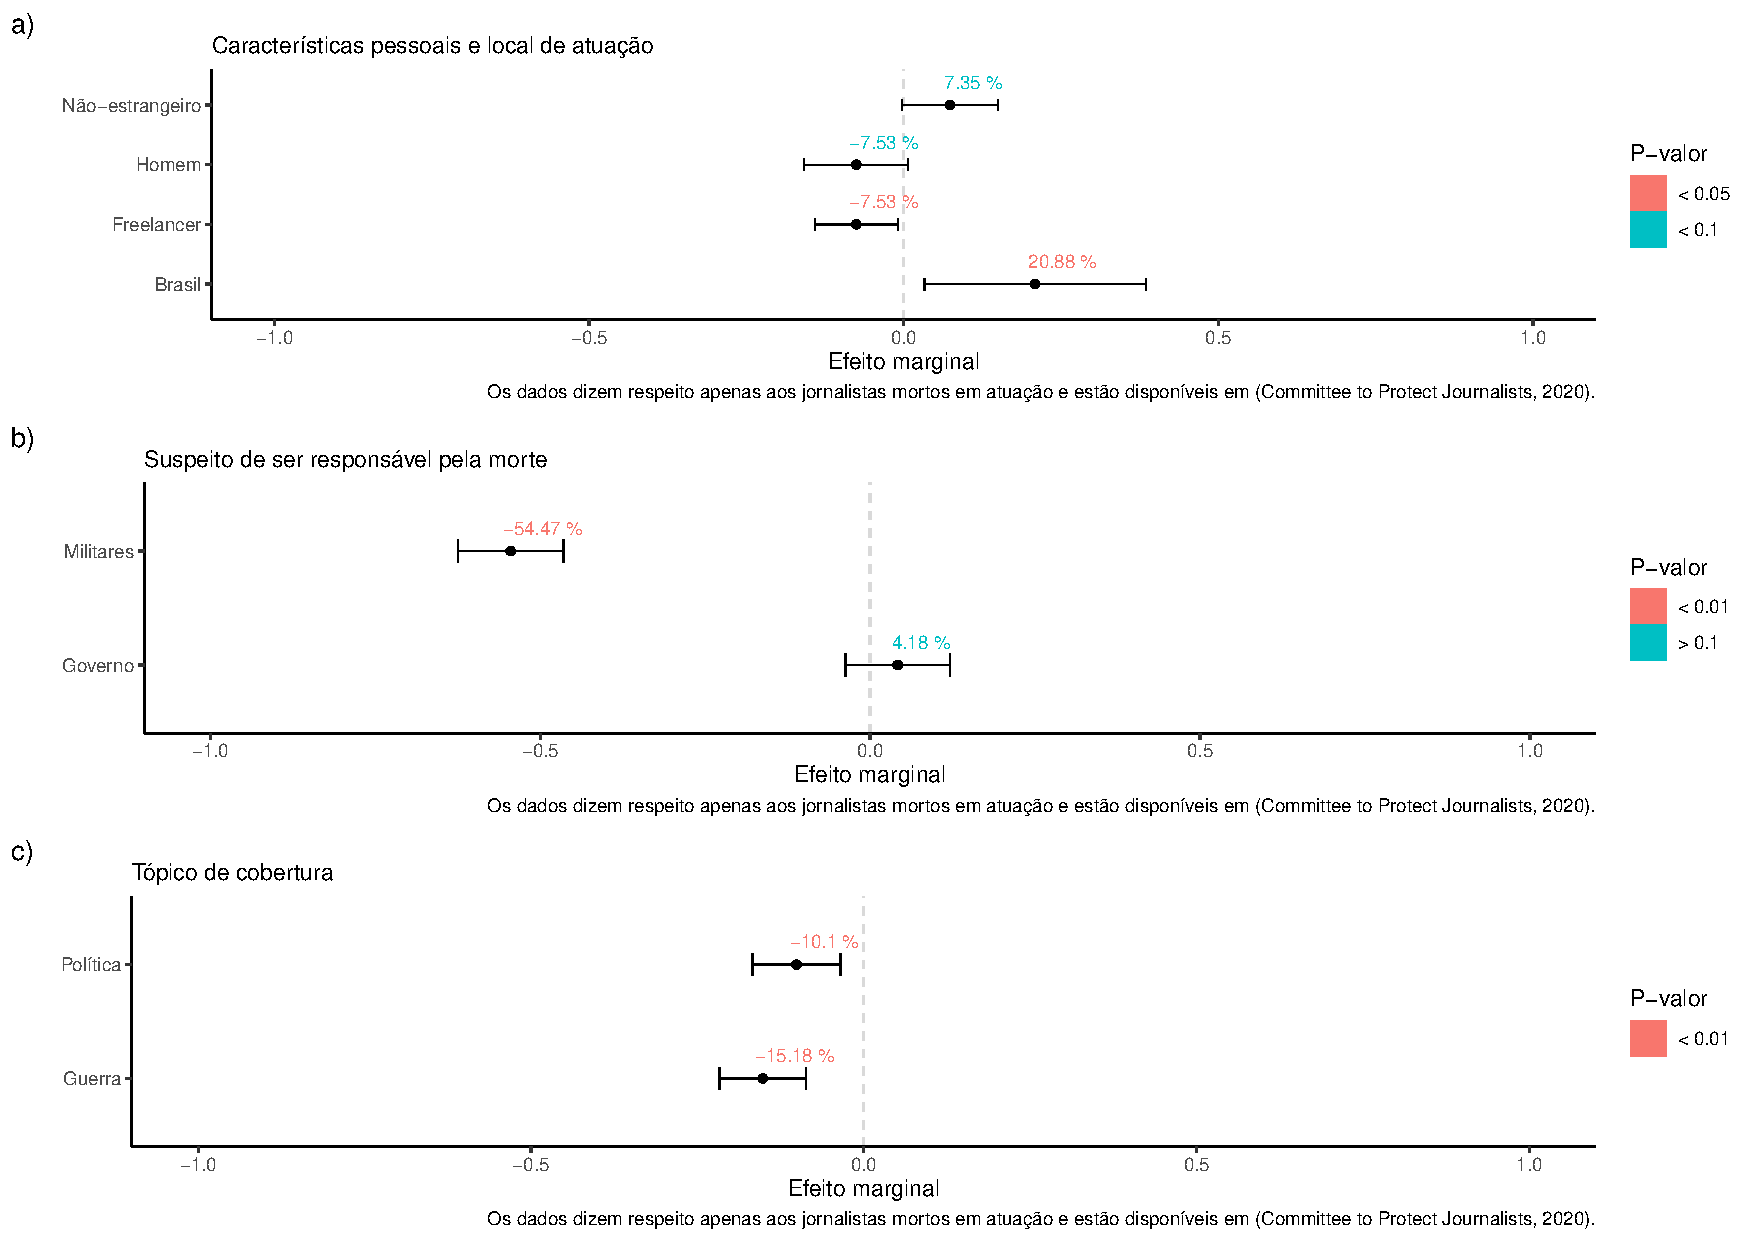
\includegraphics[width=\linewidth]{"Figuras/efeitos_marginais.pdf"} \\
\caption*{Fonte: Elaboração própria à partir dos dados disponíveis em \textit{Committee to Protect Journalists}.}
\end{figure}

\begin{figure}[H]
	\centering
	\caption{Efeitos marginais: modelo heterocedástico - probabilidades relativas de ter sido assassinado enquanto atuava}
	\label{fig:efeitos_marginais_hetprob}
	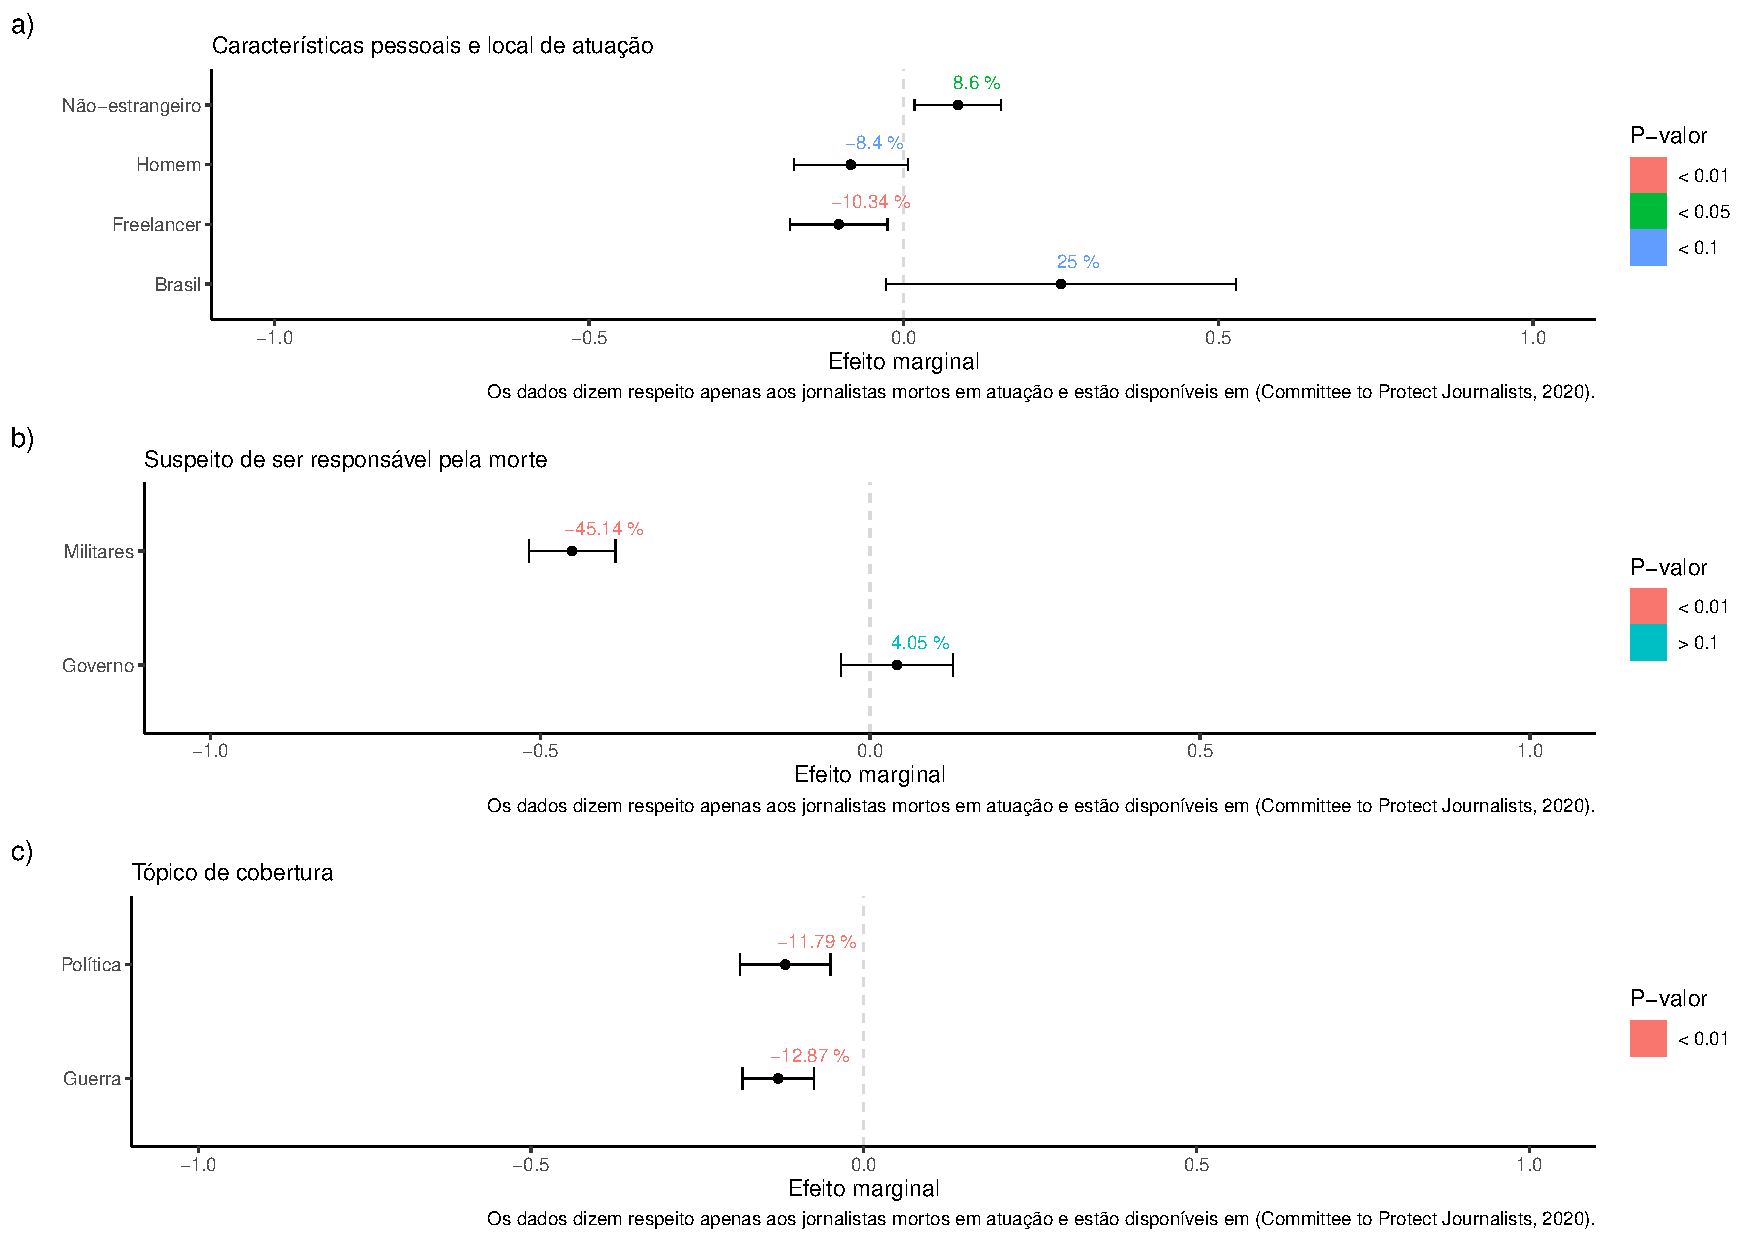
\includegraphics[width=\linewidth]{"Figuras/efeitos_marginais_hetprob.pdf"} \\
\caption*{Fonte: Elaboração própria à partir dos dados disponíveis em \cite{CPJ2020}.}
\end{figure}

Na seção seguinte são tecidas as considerações finais acerca dos resultados obtidos, bem como suas limitações e possíveis caminhos futuros para novas pesquisas.

\section{Considerações finais}

O presente trabalho teve o intuito de analisar a importância de um conjunto de variáveis que capturam características pessoais e acerca do trabalho no que tange à probabilidade de um jornalista ser assassinado em razão de sua atuação. 

De forma geral, as duas variáveis que tiveram maior relevância foram "Brasil" e "Militar", que dizem respeito ao local de atuação do profissional e ao suspeito de ter causado sua morte, respectivamente. Enquanto aqueles jornalistas que atuam no Brasil apresentam uma probabilidade $25,00\%$ maior que os demais de serem assassinados, quando a suspeita de culpa recai sobre os militares, tem-se uma redução de $45,10\%$ na probabilidade da morte ter sido um assassinato.

Em relação à robustez, acredita-se que novas especificações de formas funcionais devem ser testadas, em especial ao se considerar a grande sensibilidade do modelo Probit heterocedástico à erros de especificação. Além disso, como sugestão para novos trabalhos, recomenda-se a análise da impunidade dos crimes cometidos contra jornalistas ou de seus aprisionamentos, fazendo uso da base de dados disponível em \cite{CPJ2020}.

\bibliography{referencias.bib}

\end{document}